\documentclass[12pt,a4paper]{report}
\usepackage[italian, main=english]{babel}
\usepackage{newlfont}
\usepackage{color}
\usepackage{hyperref}
\usepackage{xcolor}
\usepackage{graphicx}
\usepackage{minted}
\usepackage{caption}

\newcommand{\source}[1]{\vspace{-5pt} \caption*{ \emph{Source}{#1}} }

\hypersetup{
    colorlinks,
    linkcolor={red!50!black},
    citecolor={blue!50!black},
    urlcolor={blue!80!black}
}

\textwidth=450pt\oddsidemargin=0pt


\begin{document}
\begin{titlepage}
\begin{center}
{{\Large{\textsc{Alma Mater Studiorum $\cdot$ Universit\`a di Bologna}}}} 
\rule[0.1cm]{15.8cm}{0.1mm}
\rule[0.5cm]{15.8cm}{0.6mm}
\\\vspace{3mm}

{\small{\bf Scuola di Scienze \\ 
Dipartimento di Fisica e Astronomia\\
Corso di Laurea in Fisica}}

\end{center}

\vspace{23mm}

\begin{center}\textcolor{black}{
{\LARGE{\bf PORTING RECONSTRUCTION \\ ALGORITHMS FOR HIGH ENERGY \\ PHYSICS USING SYCL ABSTRACTION \\ LAYER \\}}
}\end{center}

\vspace{50mm} \par \noindent

\begin{minipage}[t]{0.47\textwidth}

\large{\bf Relatore: \vspace{2mm}

{Prof. Francesco Giacomini}}

\vspace{5mm}

\large{\bf Correlatore: \vspace{2mm}

{Dott. Felice Pantaleo}}

\end{minipage}
\hfill
\begin{minipage}[t]{0.47\textwidth}\raggedleft
{\large{\bf Presentata da:
\vspace{2mm}\\
Luca Ferragina}}
\end{minipage}

\vspace{20mm}

\begin{center}
Anno Accademico 2021/2022
\end{center}

\end{titlepage}

\tableofcontents

\begin{abstract}
\begin{otherlanguage}{italian}
Nei prossimi anni è previsto un aggiornamento sostanziale di LHC, che prevede di aumentare la luminosità integrata di un fattore 10 rispetto a quella attuale. Tale parametro è proporzionale al numero di collisioni per unità di tempo. In questo contesto, risulta evidente che le risorse computazionali necessarie a tutti i livelli della ricostruzione cresceranno notevolmente. Per questo motivo, la collaborazione CMS ha cominciato già da alcuni anni ad esplorare le possibilità offerte da "heterogeneous computing", ovvero la pratica di dividere il carico di lavoro tra CPU e altri acceleratori dedicati, come ad esempio schede grafiche (GPU). Uno dei problemi principali di questo approccio è la necessita di scrivere, testare e mantenere codice diverso per ognuno dei dispositivi su cui dovrà essere eseguito. In tale contesto, questa tesi presenterà la possibilità di tradurre codice per la ricostruzione di eventi in modo che sia eseguibile e performante su diversi dispositivi senza modifiche sostanziali tramite SYCL. Quest'ultimo è un livello di astrazione open-source che rispetta lo standard ISO C++ e di cui esistono diverse implementazioni. In particolare, questo studio si concentra sul porting di un algoritmo di clustering delle energie, CLUE, usando l'implementazione SYCL supportata da Intel. Inizialmente, è stato tradotto l'algoritmo nella sua versione standalone, principalmente per prendere familiarità con il nuovo linguaggio e per la relativa comodità di confronto delle performance con le versioni native già esistenti. In questo caso, sono state testate principalmente le performance, ottenendo risultati molto simili a quelli di codice CUDA nativo eseguendo il codice sullo stesso hardware Nvidia. Per testare la fisica, l'algoritmo è stato integrato all'interno di una versione ridotta del framework usato da CMS per l'intera ricostruzione. % TODO conclusione dell'abstract
\end{otherlanguage}
\end{abstract}


\chapter*{Introduction}
\addcontentsline{toc}{chapter}{Introduction}
Research in high energy physics focuses on studying particles at the most fundamental level in order to discover how they interact. In order to gain an insight on the physical processes that involve matter at the subatomic scale, it is necessary to accelerate particles and make them collide at very high energies. The Large Hadron Collider (LHC)~\cite{LHC}, at CERN (Counseil Européen pour la Recherche Nucléaire)~\cite{CERN} accelerates protons to 14 TeV, collimating them in two parallel beams that collide at specific sites where the particle detectors are located. Four main experiments are hosted at the LHC facility: ALICE~\cite{ALICE}, LHCb~\cite{LHCb}, CMS~\cite{CMS} and ATLAS~\cite{ATLAS}, of which the latter two are general purpose experiments looking to improve our knowledge of the Standard Model~\cite{standard_model}. When protons collide at such high energies, many other particles are produced and scattered in every direction. These particles fly through the detectors and are stopped at different levels depending on their charge and energy, and can thus be identified. In high energy physics there are mainly two ways to look for new physics: either increase the energy at which particles collide, or observe more collisions to gain insight into the rarest processes. For this reason, LHC periodically undergoes a series of hardware upgrades that mainly  aim to address both the aforementioned points. In particular, the LHC is scheduled to receive a major upgrade by 2029, which will deal with both points. Firstly, the energy of the colliding beams will be increased up to the theoretical limit of the machine of 7 TeV per beam, with resulting collisions at 14 TeV in the center of mass. Secondly, the number of collisions observed per unit time (luminosity) will increase by roughly a factor 10. Because of this, detectors have to receive periodic hardware upgrades as well, to improve their sensitivity. As a result of the hardware upgrades, the statistics of each event increase as well as the amount of data to be collected and processed with very strict time requirements. To accomplish such a task, each experiment's software must be regularly updated together with the hardware. In particular, we can distinguish two kinds of algorithms used to process the data coming from the detectors: trigger and reconstruction algorithms. The first kind filters the collisions' data in real time by selecting and saving only events that satisfy particular conditions due to which they might be good candidates for new physics. Reconstruction algorithms are instead used to study these potentially interesting events by reproducing the chain of decays and interactions with the detectors that have occurred after the proton-proton collision. \newline
In this context, the CMS experiment has invested part of its resources to explore different heterogeneous computing solutions. This means that several parts of the software reconstruction can run simultaneously on different types of devices, like CPUs, GPUs or FPGAs. Recently, considerable efforts have been put in order to improve the code portability across different architectures and backends. Since writing multiple versions of the same code for each device would be extremely inefficient, some abstraction layers have been considered. In every case, the main objective is to produce an executable file that can run on many different architectures while maintaining a level of performance as close as possible to the native implementation. \newline
This thesis focuses on one of these abstraction layers, SYCL~\cite{sycl_specification}, which is based on the ISO C++ standard~\cite{iso_c++}. In particular, the porting experience of one CMS clustering algorithm from CUDA~\cite{CUDA} code, designed to run exclusively on NVIDIA GPUs, to SYCL, with a focus on the performance and physics analysis, is discussed. \newline
In Chapter~\ref{ch:1} the clustering problem in high energy physics is introduced, with a description of the CLUE algorithm, chosen for the porting experience. 
In Chapter~\ref{ch:2} the SYCL standard is presented, along with its various implementations. In particular, more details are given on Data Parallel C++, the chosen implementation to carry out the port.
Finally, in Chapter~\ref{ch:3} the porting results are shown, as well as the performance measurements.

\chapter{CLUE: a fast clustering algorithm for high energy physics}
\label{ch:1}
Prova reference\cite{CLUE}

\chapter{SYCL abstraction layer}
\label{ch:2}
\section{Standard}
\label{ch:sycl_standard}
SYCL is an abstraction layer for heterogeneous computing open source end royalty-free, maintained by Khronos Group~\cite{khronos}. At its core, SYCL proposes a more flexible and simple way to write code for multiple devices, thus improving code portability and in general, simplifying the maintenance of code. On a high level, SYCL defines a library that allows programmers to write a single source code to be executed on different devices thanks to the SYCL runtime. A standard SYCL application contains code compliant with the ISO C++ standard which can be roughly divided into host code, executed by the CPU, and device code, enclosed in $kernels$, to be executed by one or more heterogeneous devices. SYCL kernels are basically C++ function objects, so objects of some class that overload the "function call operator" \texttt{()}. For this reason, simple kernels are usually implemented as lambdas. Furthermore, device code compilation is more complicated than standard host code compilation, the added complexity is explored in the following sections. 

As previously stated, SYCL tries to be as compliant as possible with ISO C++ standards so much that all of the host code can, in theory, be compiled with a standard C++ compiler to produce an executable that can run on the CPU. This is true until any kernel is called or any OpenCL\footnote{OpenCL™ (Open Computing Language) is an open, royalty-free standard for cross-platform, parallel programming of diverse accelerators found in supercomputers, cloud servers, personal computers, mobile devices, and embedded platforms~\cite{OpenCL}.} integration is required. Some C++ features are unavailable in SYCL to guarantee the highest degree of portability across most different kinds of devices. A couple of examples are the inability to use function pointers or call virtual functions inside kernels. Furthermore, the whole error handling system is different from standard C++, mainly for the need to throw and catch asynchronous exceptions. Since heterogeneous computing is becoming increasingly more relevant year over year, Khronos is also cooperating with the C++ committee to integrate heterogeneous programming into the standard. Code~\ref{code:simple_ex} shows the basic syntax of a SYCL application.

\begin{figure}[ht!]
\renewcommand{\figurename}{Code}
\begin{minted}[linenos]{cpp}
#include <CL/sycl.hpp>

int main()
{
    // allocate input data on host
    int data[1024];
    
    // initialize sycl queue. When created, the queue is tied to a device
    auto q = sycl::queue(sycl::default_selector());
    
    // allocate memory on the device
    auto d_a = sycl::malloc_device<int>(1024, q);
    
    // copy input data from host to device
    // wait for the copy to finish at the end
    q.memcpy(d_a, &data, 1024 * sizeof(int)).wait();

    // submit task to the device
    q.submit([&](sycl::handler &cgh)
    {
        cgh.parallel_for(sycl::range<1>(N), [=](sycl::id<1> idx)
        {
            // do work on data
        });
    }).wait();
    
    // copy result data from device back to host
    q.memcpy(&data, d_a, 1024 * sizeof(int)).wait();
    
    // free device memory
    sycl::free(d_a, q);
}
\end{minted}
\caption{Sample code of a SYCL application.}
\label{code:simple_ex}
\end{figure}

Here the most important characteristics are highlighted, with some of them discussed in greater detail in the following sections. First up, the distinction between device code and host code: 
\begin{itemize}
    \item Line 19-25 is device code, every operation inside a sycl::queue::submit() will be executed on the device and the host will only take care of scheduling the work;
    \item All of the other code will be executed on the host. This includes device selection and every memory operation on it.
\end{itemize}
This separation is also tied to a different compilation model which will be explained in more detail in Section~\ref{ch:compilation_model}. On a general level, the SYCL integration starts by creating a \texttt{sycl::queue}, this object is tied to a specific device (that can be a CPU, GPU, or FPGA) and is used to manage its memory and the scheduling of jobs to be executed on it. Memory on the device is allocated through the \texttt{sycl::malloc\_device} function and freed using \texttt{sycl::free}. Note that in both cases a queue has to be provided to get the context and device on which to allocate or free the memory. Finally, note that after each queue operation there is an explicitly \texttt{wait} used to synchronize the completion of the kernel. Data dependencies and synchronization are discussed at length in Section~\ref{ch:synchronization}. In general, this is not strictly necessary, depending on the goals and structure of the program.

\section{Implementations}
\label{ch:sycl_implementations}
Being an open-source, royalty-free, project means that SYCL has many different implementations which all support different backends. The main SYCL implementations are schematically reported in Figure~\ref{fig:sycl_implementations}.

\begin{figure}[H]
    \centering
    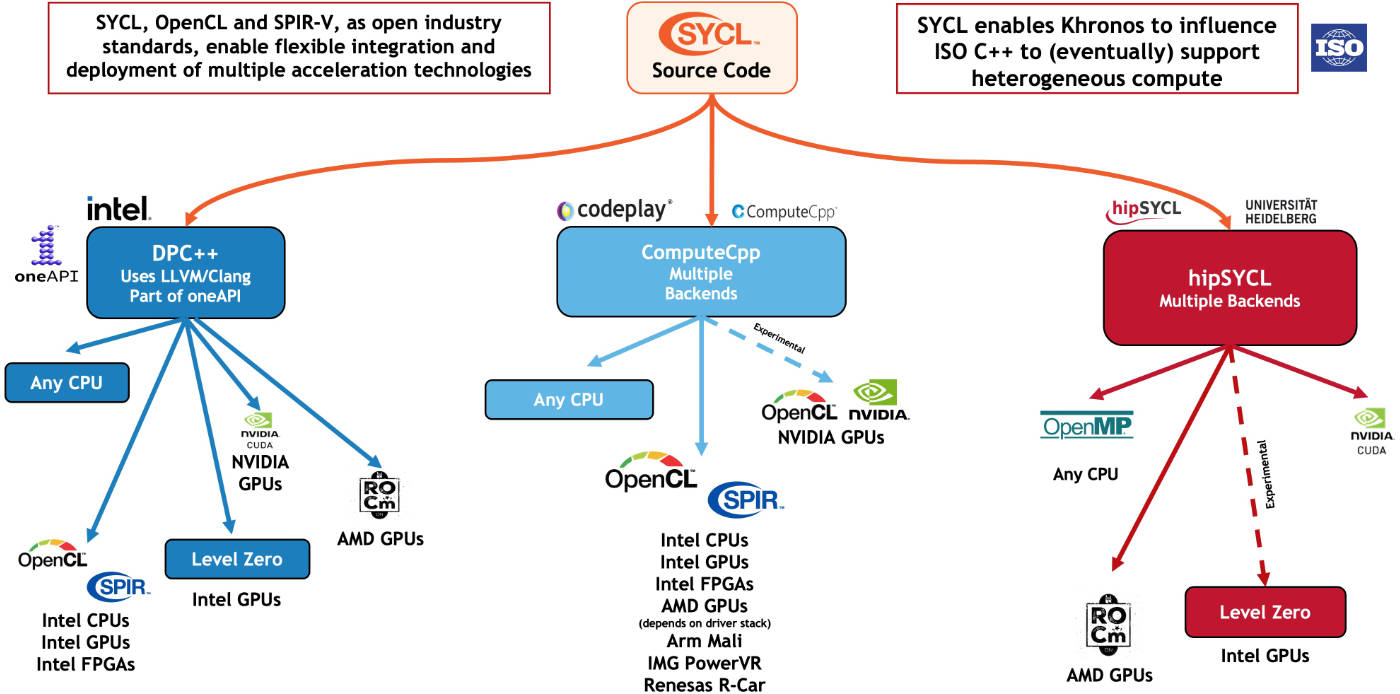
\includegraphics[width=0.9\textwidth]{media/sycl_implementations.jpg}
    \caption{Overview of the main SYCL implementations.}
    \source{\emph{:}\cite{khronos}}
    \label{fig:sycl_implementations}
\end{figure}

In general, as of SYCL 2020, an implementation is made of four different components, represented in Figure~\ref{fig:sycl_implementations_backend}: 
\begin{itemize}
    \item SYCL interface: a template library that provides the developers with the features of SYCL; 
    \item SYCL runtime: the library that schedules and executes work on both the host and devices. Specifically, it schedules memory operations, launches kernels, and tracks data dependencies;
    \item Backend interface: point of contact between the SYCL runtime and a specific device. Some examples of backends are OpenCL (used to interface with CPUs), CUDA (used to interface with NVIDIA GPUs), Level Zero (used to interface with Intel GPUs), and HIP/ROCM (used to interface with AMD GPUs). Not all backends are supported in all the implementations. 
    \item SYCL device compiler: C++ compiler used to identify SYCL kernels and compile them down to an Intermediate Representation (IR) to then be linked with code compiled by the host compiler.
\end{itemize}

\begin{figure}[H]
    \centering
    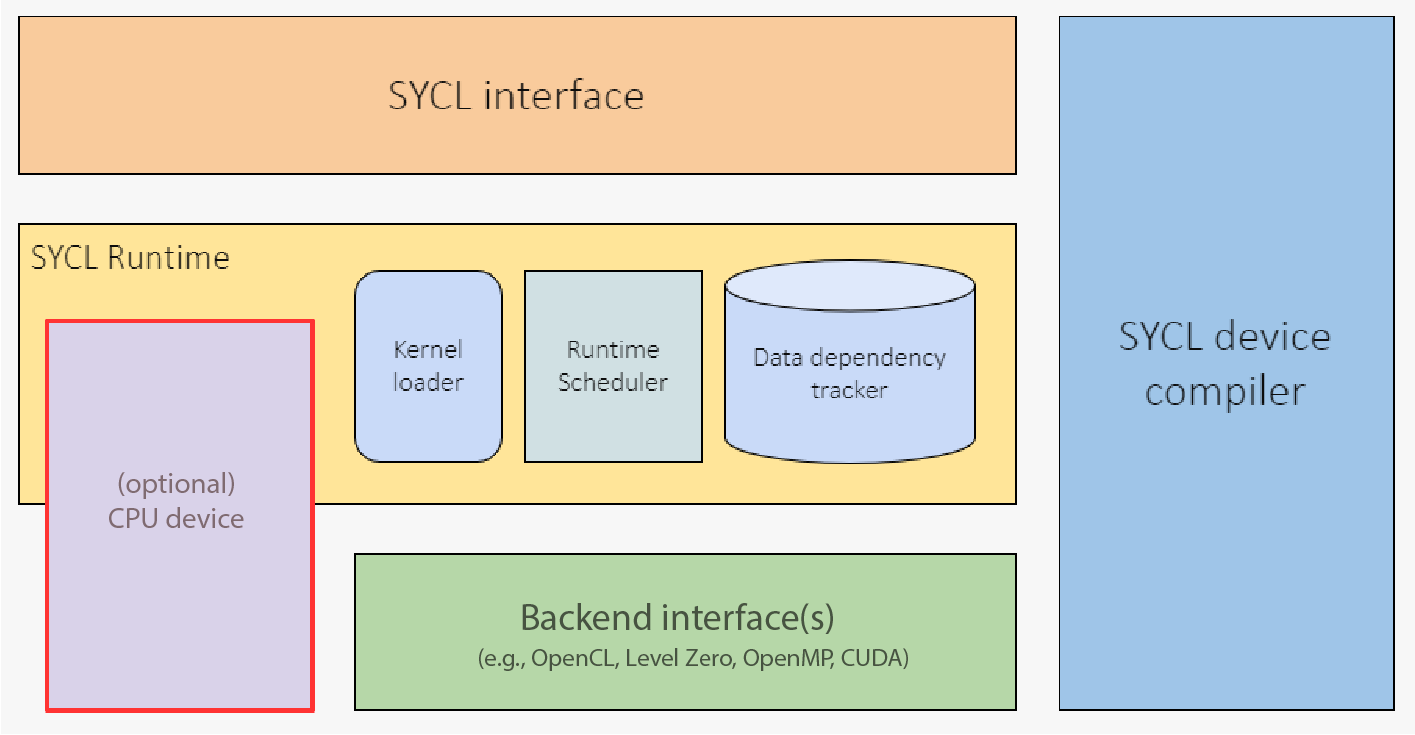
\includegraphics[width=\textwidth]{media/ex_sycl_implementation.png}
    \caption{Schematic representation of the SYCL implementation backend interface.}
    \source{\emph{:}\cite[lesson 1 - slide 12]{syclacademy}}
    \label{fig:sycl_implementations_backend}
\end{figure}

\subsubsection{OneAPI and Data Parallel C++}
Data Parallel C++ is the SYCL implementation developed by Intel and integrated into oneAPI, their toolkit for heterogeneous programming~\cite{oneAPI}. This implementation is compliant with the SYCL 2020 standard and thus supports the Universal Shared Memory model, as described in Section~\ref{ch:memory_management}. oneAPI includes a low-level hardware interface known as Level Zero. This backend interfaces directly with the SYCL runtime and is used to execute code on Intel GPUs and FPGAs that support it. As far as other backends are concerned, oneAPI officially supports OpenCL to interface with CPUs and its support for CUDA is under development. Its native support for USM and the auxiliary tools provided, as well as native support for Intel hardware, are what ultimately brought CMS to choose this specific SYCL implementation to explore its capabilities in high-energy physics software reconstruction. A particular highlight is a support tool for developers who are first exploring SYCL capabilities. Included in oneAPI, there is a compatibility tool, Data Parallel Compatibility Tool (DPCT), which can automatically convert CUDA code into SYCL code. While the output from the tool is not always correct and some specific functions or features are not translated entirely, the compatibility tool surely helps to lay the groundwork to move from CUDA code to SYCL code, easing the refining work that needs to be done by the developer.
The Data Parallel C++ compiler, \texttt{dpcpp}, is regularly forked from the open source LLVM project~\cite{dpcpp}.

\section{Compilation model}
\label{ch:compilation_model}
SYCL follows a single-source, multiple-pass compilation model. Since the source code is just one, the kernels are standard C++ function objects\footnote{In C++, a function object is a generic class which implements an overload of the operator function call \texttt{()}.}, generally implemented as lambda expressions. Because host and device codes are different, the code passes through a compiler twice: first through the host compiler to produce a CPU object and then through the device compiler. This second pass on the device code produces a device IR for the specific architecture of the targeted device. Finally, the CPU object is linked with the IR to produce a single executable with code for both the CPU and the device. What was just described is generally known as the Ahead of Time (AoT) compilation model. The SYCL implementation chosen to carry out the porting, oneAPI, also allows compiling only the host code while not targeting any specific device. In this case, the device code will be compiled only at run time using the Just in Time (JiT) compiler. This gives the user more flexibility to run on many different supported devices while not necessarily having access to a compiler or compiled code for a specific device or architecture (as long as both are supported by the implementation).

\section{Execution model}
\label{ch:execution_model}
Every SYCL device is divided into multiple Compute Units (CUs) which are in turn split into Processing Elements (PEs). Every kernel computation will be executed on the PEs of the relevant device. When a kernel is launched, a thread hierarchy gets initialized. The main element in a SYCL thread hierarchy is the ND-range, which is a 1, 2, or 3-dimensional grid of work groups, that are equally sized groups of the same dimensionality. These work groups are in turn divided into work items, as shown in Figure~\ref{fig:sycl_nd_range}. Diving into the single elements of the hierarchy, in SYCL, the programmer has access to:
\begin{itemize}
    \item Work item: a single thread within the thread hierarchy;
    \item Work-group: a 1, 2 or 3-dimensional set of threads (work-items) within the thread hierarchy;
    \item ND-range: it's the representation of the thread hierarchy used by the SYCL runtime when executing work. It has three components: the global range, the local range, and the number of work groups. The global range is the total number of work items within the thread hierarchy in each dimension; the local range is the number of work items in each work group in the thread hierarchy, and the number of work groups is the total number of work groups in the thread hierarchy, which can be derived from the global and local.
\end{itemize}

\begin{figure}[ht!]
    \centering
    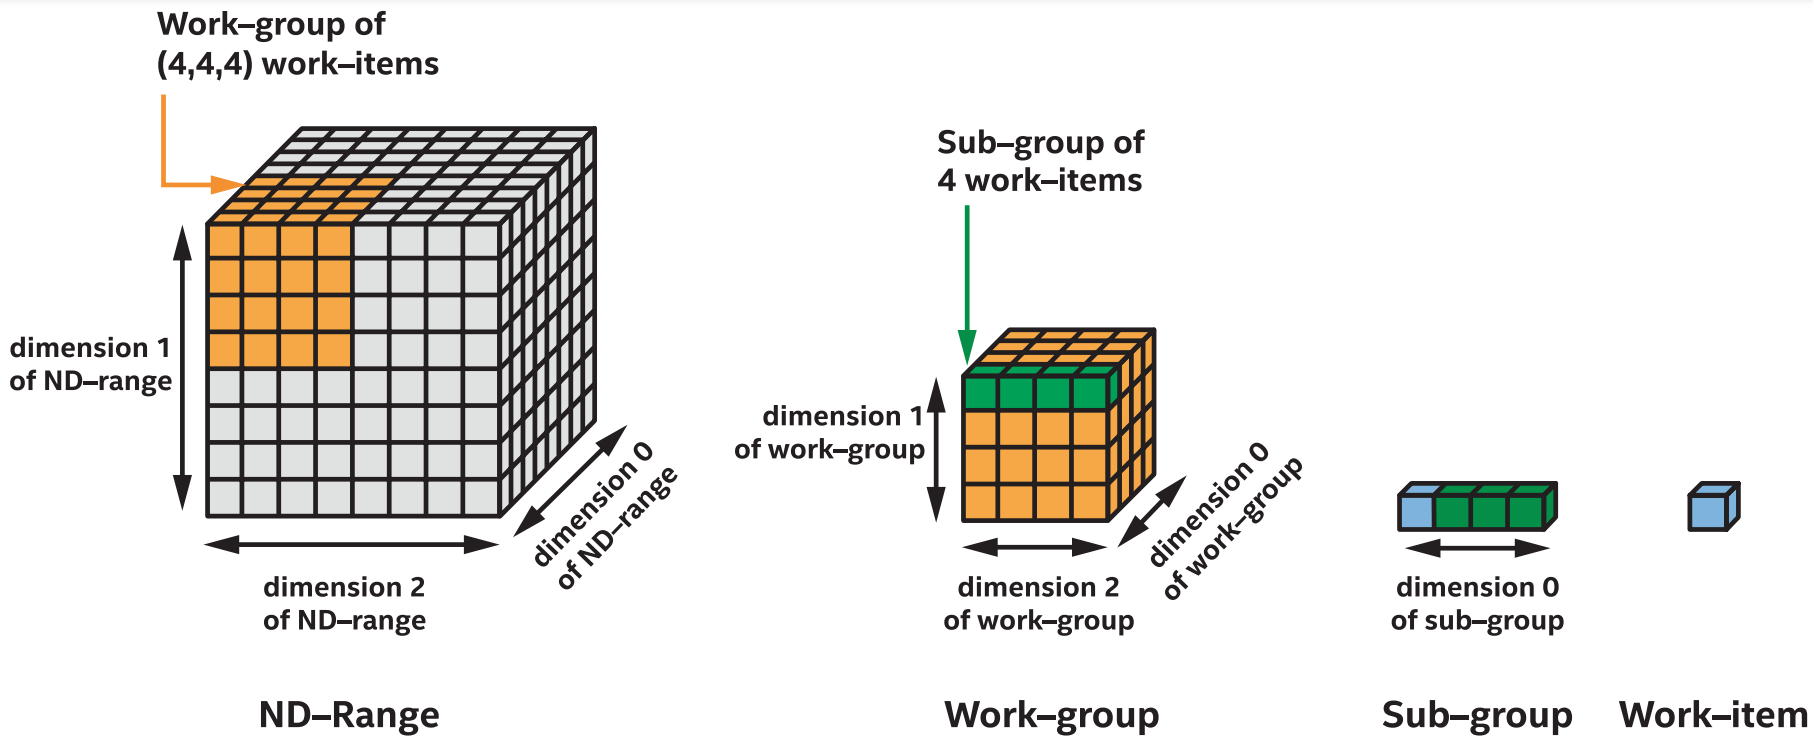
\includegraphics[width=\textwidth]{media/sycl_nd_range.png}
    \caption{Pictorial representation of the SYCL thread hierarchy.}
    \label{fig:sycl_nd_range}
\end{figure}

On some modern hardware platforms, there is also the possibility of accessing subsets of the work items in a
work-group to execute them with additional scheduling guarantees. These subsets are known as sub-groups. 

In SYCL, the work-group size can be left empty, and then implementation can set it to the optimal value according to an internal heuristic. Additionally, SYCL does provide a mechanism to get the preferred work-group size. An example of how to do it is shown in Code~\ref{code:work_group_size}. Typically, choosing a work group size that is a multiple of the preferred one will be enough.

\begin{figure}[ht!]
\renewcommand{\figurename}{Code}
\begin{minted}[linenos]{cpp}
auto pWGSM = kernel.get_work_group_info<
sycl::info::kernel_work_group::preferred_work_group_size_multiple>();

queue.submit([&](sycl::handler &cgh){
    cgh.parallel_for(kernel, sycl::range<1>(pWGSM), 
                     [=](sycl::id<1> idx){
        /* kernel code */
      });
  });
\end{minted}
\caption{Query of preferred work-group size for a specific kernel.}
\label{code:work_group_size}
\end{figure}

\subsection{Memory management}
\label{ch:memory_management}
SYCL is based on the OpenCL memory model but operates at a higher level of abstraction, which means that storage and access memory are separated and treated with different objects: buffers and accessors, respectively. SYCL buffers are, at their core, \texttt{std::unique\_ptr} wrapped in such a way to make them live only inside the scope they are defined in. The buffer manages memory allocation/copy, while accessors create requirements on the buffers. These requirements can be allocating memory, synchronization between different accessors or data transfer between host and device. Depending on the accessor, data is automatically allocated on the host or on the device. In the more recent SYCL specification, a big push has been made to allow explicitly allocating memory using C-like pointers. This method offers greater flexibility by allowing the programmer to explicitly allocate and copy exactly when they intend to, often reducing memory overhead. In order to allocate using regular pointers, the device has to support Universal Shared Memory (USM). Furthermore, SYCL operates in three different memory spaces: 
\begin{itemize}
    \item Private memory: region of memory allocated per work item and only visible to that work item. Cannot be accessed from the host;
    \item Local memory: contiguous region of memory allocated per work group and visible to all of the work items in that work-group. This memory is allocated and accessed using an accessor and cannot be accessed from the host;
    \item Global memory: a memory visible by all of the work groups of the device.
\end{itemize}

\begin{figure}[H]
\centering
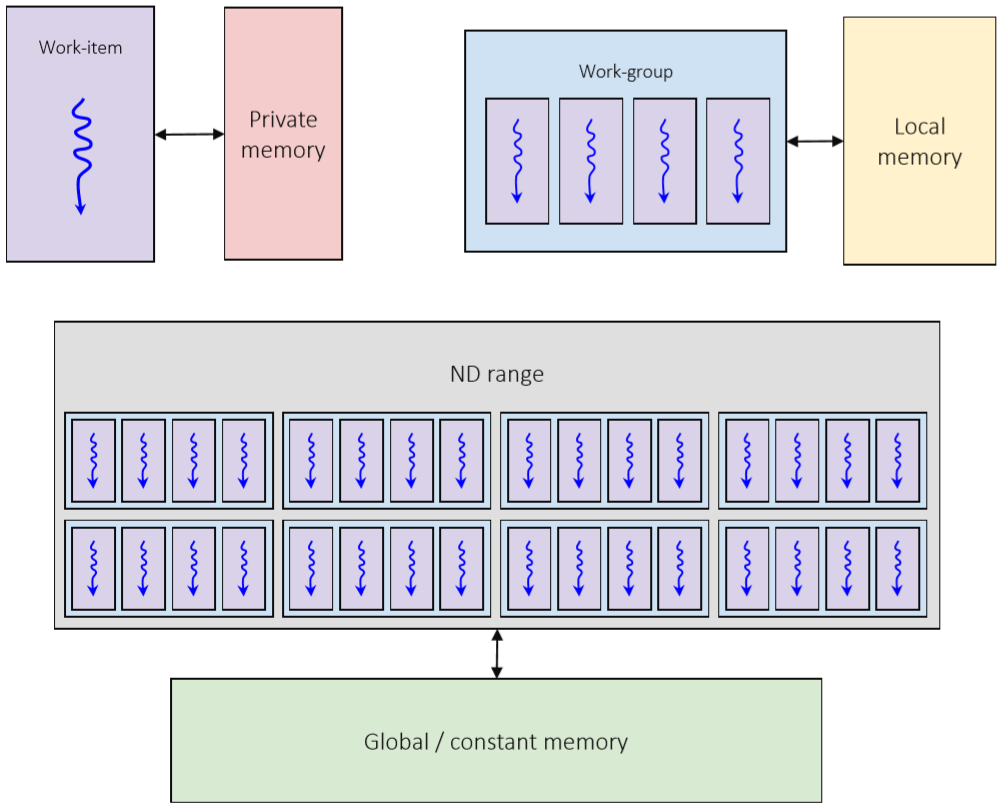
\includegraphics[width=0.9\textwidth]{media/sycl_memory_layout.png}
\caption{SYCL memory layout.}
\source{\emph{:} SYCL Academy~\cite[Lesson 4 - slide 6]{syclacademy}}
\label{fig:nd-range-mem}
\end{figure}

Explicit allocation of memory through pointers has still some limitations like the inability to specify whether the allocation should be in private or local memory and defaults to private. However, this fairly new feature is still been worked on and improvements can be expected in the next SYCL releases.

\subsubsection{Memory allocation and transfer}
Due to the previously mentioned efficiency reasons, this work has been carried out entirely using the USM model. In this case, memory allocation is done through the \texttt{sycl::malloc} function which is divided into three different methods:

\begin{itemize}
    \item \texttt{malloc\_host}: allocate memory on the host that is accessible on both the host and the device. These allocations cannot migrate to the device’s attached memory so kernels that read from or write to this memory do it remotely, often over a slower bus such as PCI-Express;
    \item \texttt{malloc\_device}: device allocations that can be read from or written to by kernels running on a device, but they cannot be directly accessed from code executing on the host. Data must be copied between host and device using the explicit USM memcpy mechanisms;
    \item \texttt{malloc\_shared}: like host allocations, shared allocations are accessible on both the host and device, but they are free to migrate between host memory and device-attached memory automatically.
\end{itemize}

Memory allocated through these methods needs to be managed using specific SYCL functions:

\begin{itemize}
    \item \texttt{sycl::queue::memset(ptr, value, num\_bytes)}: Set \texttt{num\_bytes} of memory allocated using malloc functions to \texttt{value};
    \item \texttt{sycl::queue::memcpy(dest, src, num\_bytes)}: Copies \texttt{num\_bytes} from \texttt{src} to \texttt{dest};
    \item \texttt{sycl::free(ptr, queue)}: Frees memory located at \texttt{ptr} and previously allocated usign a SYCL malloc function.
\end{itemize}

Excluding the last method, the other twp are also available as methods of the \texttt{sycl::handler} class, so they can be used inside a \texttt{queue::submit()} scope as demonstrated in Code~\ref{code:handler_copy}.


\begin{figure}[ht!]
\renewcommand{\figurename}{Code}
\begin{minted}[linenos]{cpp}
q.submit([&](sycl::handler &h) {
    // copy hostArray to deviceArray
    h.memcpy(device_array, &host_array[0], N * sizeof(int));
    });
q.wait();
\end{minted}
\caption{Example of explicit memory copy using a sycl handler.}
\label{code:handler_copy}
\end{figure}

Note that in order to allocate and deallocate in SYCL it is necessary to have declared a queue first, as to choose the device on which each memory operation should be executed. Furthermore, since copying is asynchronous by default, it is a good practice to always use \texttt{sycl::queue::wait()} after any group of copying actions to prevent segmentation faults or unexpected behaviours. Finally, in SYCL it is not necessary to specify the direction of copying (host-device, device-device, device-host) as it is deduced at run time. The usage of the discussed methods is exemplified in Code~\ref{code:sycl_memory}.

\begin{figure}[ht!]
\renewcommand{\figurename}{Code}
\begin{minted}[linenos]{cpp}
std::vector<float> h_a(N);
auto queue = sycl::queue{sycl::default_selector{}};
auto d_a = sycl::malloc_device<float>(N, queue);
auto d_b = sycl::malloc_device<float>(N, queue);

queue.memset(d_a, 0x00, N * sizeof(float));
queue.memset(d_b, 0x00, N * sizeof(float));

queue.memcpy(d_a, h_a.data(), N * sizeof(float));
queue.memcpy(d_b, d_a, N * sizeof(float));
queue.memcpy(h_a.data(), d_b, N * sizeof(float)).wait();

sycl::free(d_a, queue);
sycl::free(d_b, queue);
\end{minted}
\caption{Code sample for SYCL memory management methods.}
\label{code:sycl_memory}
\end{figure}

\subsection{Kernels execution}
\label{ch:kernels_execution}
SYCL kernel functions are called using one of the following invoke API entries (which are methods of SYCL handlers):
\begin{itemize}
    \item \texttt{single\_task}: The kernel function is executed exactly once;
    \item \texttt{parallel\_for}: The kernel function is executed ND-range times passing thread identification objects as parameters.
\end{itemize}
Examples for both of these kernels' calls are shown in Code~\ref{code:kernel_execution}.

\begin{figure}[ht!]
\renewcommand{\figurename}{Code}
\begin{minted}[linenos]{cpp}
// execute the kernel function exactly once
auto queue = sycl::queue(sycl::default_selector{})
queue.submit([&](sycl::handler& h)
             {
                 h.single_task([=]{a[0] = 1.0f});
             });
             
// execute the kernel function nd-range times
auto queue = sycl::queue(sycl::default_selector{})
queue.submit([&](sycl::handler& h)
             {
                h.parallel_for(range, [=](id<1> i) {a[i] = b[i]}); 
             });
\end{minted}
\caption{Examples of SYCL kernel calls.}
\label{code:kernel_execution}
\end{figure}

The handler defines the interface to invoke kernels by submitting commands to a queue.
A handler can only be constructed by the SYCL runtime and is passed as an argument to the command group function. The command group function is an argument to submit.

The SYCL kernel function invoke API takes a C++ callable object by value which is most often expressed as a lambda. If local memory is required or work-group size is specified manually, then the corresponding \texttt{nd\_range} object must be used as the first parameter. In turn, the \texttt{nd\_item} associated with the \texttt{nd\_range} can be passed inside the kernel and its method for barriers or work-group operation can be used.


One tricky issue found when dealing with SYCL kernels is that, as per SYCL specification~\cite{sycl_specification}, variables can be passed inside a kernel (\texttt{parallel\_for}) only by value, furthermore the capture of *this is not allowed neither implicitly nor explicitly (in general, this would point to host memory which is not accessible on the device). To resolve this issue you can simply create local copies of all the variables needed inside the kernel before the \texttt{parallel\_for} gets called, as shown in Code~\ref{code:kernel_variables}.

\begin{figure}[ht!]
\renewcommand{\figurename}{Code}
\begin{minted}[linenos]{cpp}
sycl::queue q = sycl::queue(sycl::default_selector{});
q.submit([&](sycl::handler& h)
{
    auto var_kernel = var;
    h.parallel_for(...,[=](...)
    {
        /* use var_kernel here */               
    });
});
\end{minted}
\caption{Example of queue submission using a multidimensional range.}
\label{code:kernel_variables}
\end{figure}

\subsection{Synchronization}
\label{ch:synchronization}
SYCL provides a single synchronization level that is across all of the work items within a single work group using barriers that can be called inside kernels.
\begin{itemize}
    \item \texttt{mem\_fence}: inserts a memory fence on global memory access or local memory access across all work items within a work group.
    \item \texttt{barrier}: like the previous one, but it also blocks the execution of each work item within a work group at that point until all of them have reached that point.
\end{itemize}
In Code~\ref{code:item_barriers} synchronization between work-items is demonstrated using a snippet from a parallel reduction kernel.

\begin{figure}[ht!]
\renewcommand{\figurename}{Code}
\begin{minted}[linenos]{cpp}
sycl::queue q = sycl::queue(sycl::default_selector{});
unsigned int tid = item.get_local_id(0);
unsigned int i = item.get_group(0) * item.get_local_range().get(0) 
                 + item.get_local_id(0);

sdata[tid] = input[i];

item.barrier();
\end{minted}
\caption{Synchronization between work-items within the same work-group. In this example, consider sdata as an array in local memory. This snippet needs to be inside a \texttt{parallel\_for} scope to have access to the \texttt{sycl::item} used for synchronizing.}
\label{code:item_barriers}
\end{figure}

SYCL does not provide any memory fences or barriers across the entire kernel, only across the work items within a work group.

As previously noted and shown in Code~\ref{code:simple_ex}, memory operations, in particular memory copies, and kernel execution in SYCL are asynchronous by default. This means that by just scheduling a particular operation, it is not guaranteed that it will be executed before any other unless relevant data dependencies are specified by the programmer. To be more specific, SYCL queues are by default not in order, meaning that different kernels (i.e. \texttt{queue::submit()}) can and will be executed at the same time whenever possible to improve performance.
If the data used by different kernels is not independent, the queue should be initialized as in-order by passing an extra argument in the constructor as shown in Code~\ref{code:in_order_queue}.

\begin{figure}[ht!]
\renewcommand{\figurename}{Code}
\begin{minted}[linenos]{cpp}
// create a default queue
// kernels will be executed in such a way to 
// maximize parallel execution
auto q = sycl::queue(sycl::default_selector());

// create an in-order queue
// kernels will be executed in the order they
// are scheduled
auto q2 = sycl::queue(sycl::default_selector(),
                      sycl::property::queue::in_order());
\end{minted}
\caption{Creating a queue defaults to an out-of-order one. Kernels can be executed sequentially when the queue is created specifying the in-order property.}
\label{code:in_order_queue}
\end{figure}

Using an in-order queue corresponds to adding a \texttt{sycl::queue::wait()} after each and every submission. In this way, operations are executed in issue order on the selected device.

In case the code allows for some kernels to be executed in parallel while others have explicit dependencies, it is possible to use a default queue and specify the desired data dependencies using the member function \texttt{sycl::handler::depends\_on()} which can take an event or an array of events as parameters, as shown in Code~\ref{code:depens_on}. Note that, in this particular example, the second submit has an explicit dependency on the first, so the queue will wait and synchronize before executing it. However, the last submission can be executed at the same time as the first one since no data dependency is specified.

\begin{figure}[ht!]
\renewcommand{\figurename}{Code}
\begin{minted}[linenos]{cpp}
// initialize an out-of-order queue
auto q = sycl::queue(sycl::default_selector{});
// define an event
auto e = q.submit([&](sycl::handler& h)
                  {
                      /* kernel */
                  }
q.submit([&](sycl::handler& h)
         {
             h.depends_on(e);
             /* kernel */
         });
q.submit([&](sycl::handler& h)
         {
             /* kernel */
         })
\end{minted}
\caption{In-order kernel execution using explicit data dependencies.}
\label{code:depens_on}
\end{figure}

\chapter{Porting CLUE to SYCL}
\label{ch:3}


\chapter*{Conclusions and future work}
\addcontentsline{toc}{chapter}{Conclusions and future work}

\chapter*{Acknowledgements}
\addcontentsline{toc}{chapter}{Acknowledgements}

\chapter*{Bibliography}
\addcontentsline{toc}{chapter}{Bibliography}
\bibliographystyle{IEEEtran}
\bibliography{ref}
\end{document}
